\chapter{Mesh generation}
\section{Defining dimensions}
In order to initialize the structure of the Double Quantum Dot, in the \texttt{dqdfdsoi.geo} file are defined the main dimensions that caracterize the device:\\
First, the dimensions of the domain along the x direction are defined through the variable \texttt{domain\_width} and \texttt{channel\_width}, where the latter is
the width of the portion of the device where the quantum dots will be defined. The dimensions are set equal to 60nm and 40nm, respectively.\\

Then, along the y direction, the lenghts of the plunger gates, barrier gates, source/drain and the gaps between them are defined, which are summerized in the following scheme (\ref{qdoty}):
\begin{figure}[h]
\center
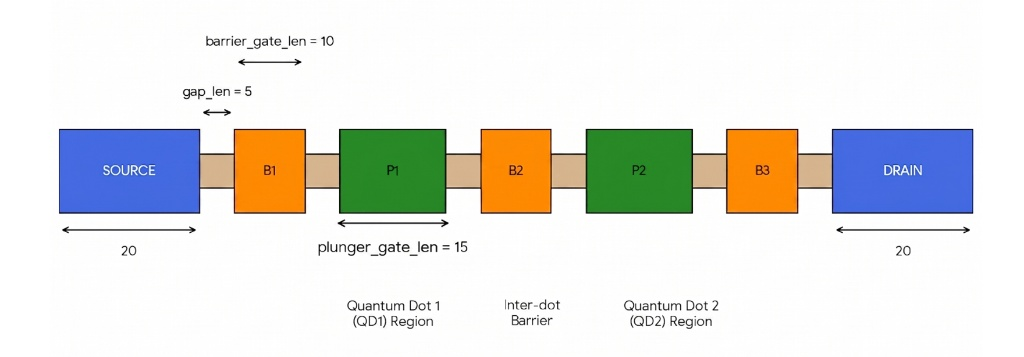
\includegraphics[width=0.8\textwidth, height=0.3\textwidth]{leo_part/dqdot_y.jpeg}
\caption{Scheme of the double quantum dot structure along the y direction, all the dimensions are in nm.}
\label{qdoty}
\end{figure}

Finally, the thicknesses along the z direction of the different layers. Starting from the bottom of the device, we have in order:
\begin{itemize}
    \item \texttt{box\_thick}: set equal to 10nm, it is the thickness of the oxide below the silicon structure;
    \item \texttt{film\_thick}: set equal to 10nm, represents the thickness of the silicon layer where the quantum dots will be formed;
    \item \texttt{gate\_oxide\_thick}: set equal to 2nm, it is the thickness of the oxide layer below the gates.
\end{itemize}


\section{Mesh structures and solids}
The geometry is constructed by defining several rectangles that represent the functional parts of the Double Quantum Dot. The command used is \texttt{Rectangle(tag) = \{x, y, z, dx, dy\}}, where the coordinates define the lower-left corner and \texttt{dx, dy} the dimensions. 
First, a rectangle is defined to represent the main domain of the simulation and above it the rectangles representing source, drain and the channel are costructed.
Then, a sequence of rectangles is generated through a \texttt{For} loop to define the barrier and plunger gates. These rectangles initially overlap with the main channel and the simulation domain. To ensure a conformal mesh (where nodes match perfectly at the interfaces), the \texttt{BooleanFragments} command is applied. This operator "slices" all the surfaces at their intersections, creating a mosaic of non-overlapping pieces.

Solids are defined through \textbf{Extrusion}. This process takes a 2D surface and "pushes" it along the z-axis, automatically creating the volume and the lateral boundary surfaces.
In our simulation, this method is used to create the oxide layer below the gates, through the line:\\ \texttt{Extrude \{0, 0, gate\_oxide\_thick\} \{Surface\{2:36\}; Layers \{2\};\}}, where the surfaces from 2 to 36 represents the surfaces generated after the \texttt{BooleanFragments} command and \texttt{Layers\{2\}}  explicitly divides the thickness of the extruded volume into two layers of prismatic elements for the subsequent mesh generation. This ensures that the mesh nodes are consistently aligned along the z-direction, providing the minimum vertical resolution required for the numerical convergence of the Poisson and Schrödinger solvers.
However, one could define a solid manually without extrusion by following these steps:
\begin{enumerate}
    \item Define the \textbf{Surfaces} that form the boundary of the object;
    \item Group these surfaces into a \textbf{Surface Loop}, which represents a closed shell;
    \item Define a \textbf{Volume} by referencing the ID of the Surface Loop.
\end{enumerate}
In our case, the extrusion is the most efficient method because it guarantees that the volumes of the different parts of the device are perfectly stacked and aligned.

\section{File formats and export}
At the end of the script, the structure is saved in two different formats, each serving a specific purpose in the QTCAD workflow:

\begin{itemize}
    \item \textbf{.msh2 (Gmsh Mesh Version 2.0):} This is the standard file format for storing the generated mesh (nodes, elements, and physical groups). It is the file that the QTCAD solver will actually read to perform the finite element calculations. The version 2.0 is often preferred for compatibility with various scientific libraries.
    \item \textbf{.geo\_unrolled:} This is a "flat" version of the geometry script. Since the original code uses loops (\texttt{For}) and variables, the unrolled version expands everything into raw, explicit Gmsh commands. It is extremely useful for debugging, as it allows the user to see exactly which tags and IDs were assigned to every single point, line, or surface created during the generation process. However, The use of the \texttt{OpenCASCADE} kernel and advanced boolean operations like \texttt{BooleanFragments} leads to a \texttt{.geo\_unrolled} file that contains a \texttt{Merge} command pointing to a \texttt{.xao} file, where Gmsh serializes the internal CAD state into the \texttt{.xao} (OpenCASCADE ASCII) format, which stores the Boundary Representation (B-Rep) of the fragmented structure.
\end{itemize}

\newpage
\section{Mesh generation and visualization}
After executing the Gmsh script, several files are automatically generated in the working directory:
\begin{itemize}
    \item \textbf{dqdfdsoi.msh2:} The primary output file containing the discretized geometry (nodes and elements) and the mapping of physical groups.
    \item \textbf{dqdfdsoi.geo\_unrolled:} A flattened version of the input script where all loops and variables are resolved.
    \item \textbf{dqdfdsoi.geo\_unrolled.xao:} An OpenCASCADE-specific file, since we used the OpenCASCADE factory.
\end{itemize}
As discussed previously, the \texttt{.geo\_unrolled} file in this case does not show the individual points and lines but rather a \texttt{Merge} command of the \texttt{.xao} file.

\section{Dimensions and Geometric Analysis}
\begin{figure}[H]
    \center  
    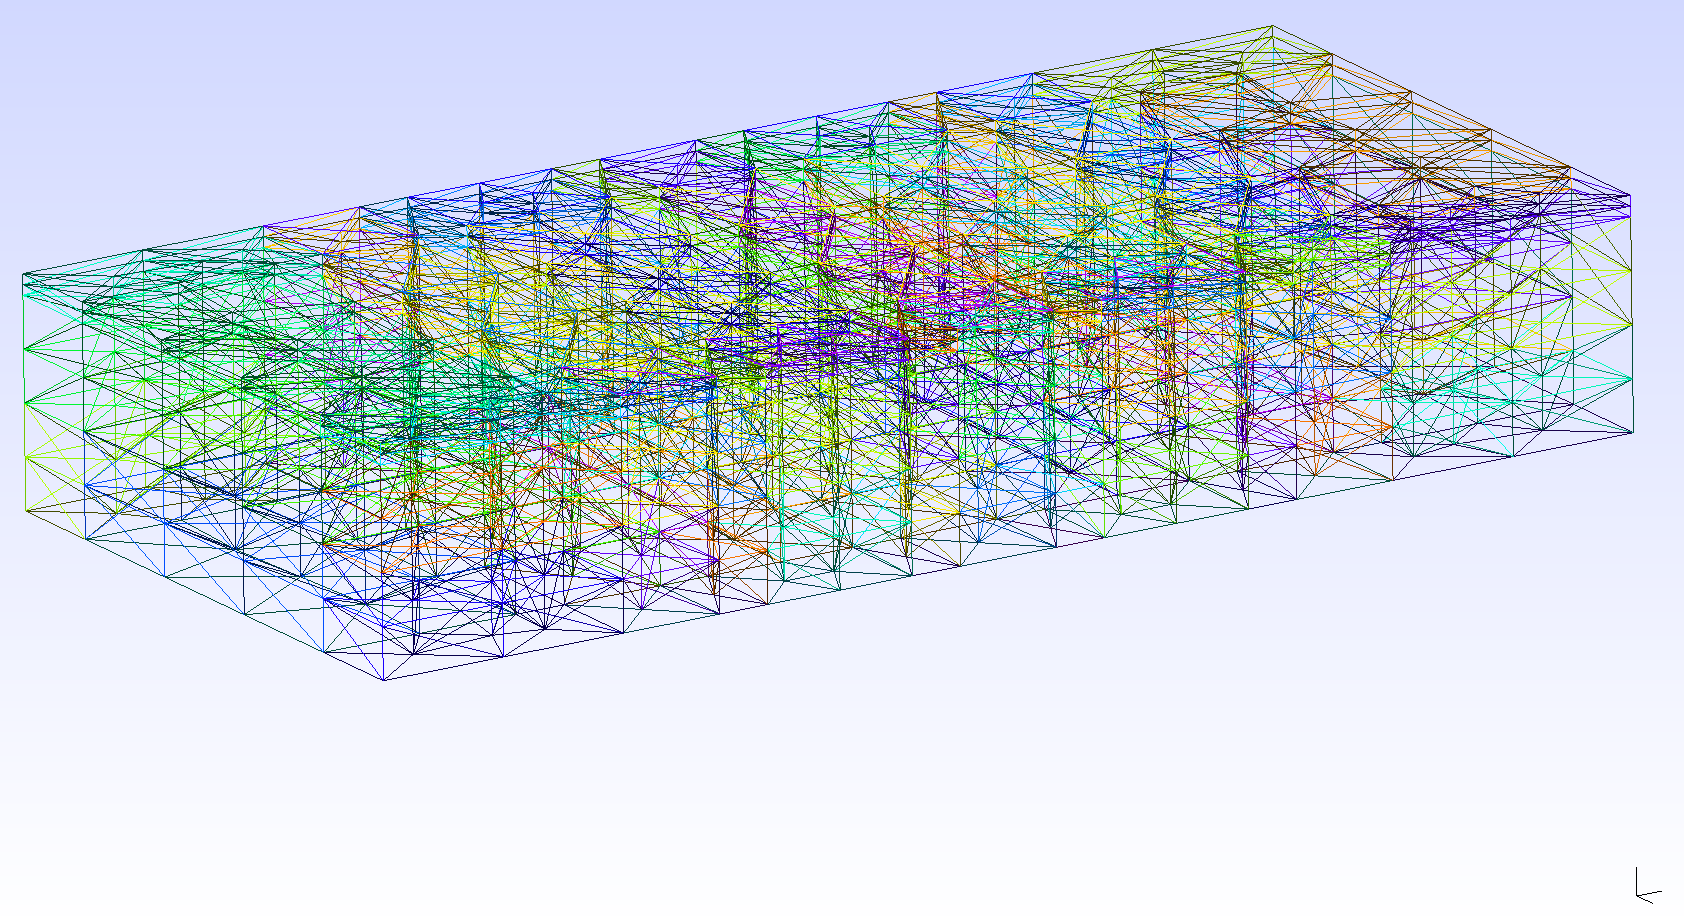
\includegraphics[width=0.7\textwidth]{leo_part/mesh_imag.png}
    \caption{Image of the resulting mesh of the device}
    \label{mesh_figure}
\end{figure}
The total dimensions of the device are determined by the combination of all previouslydefined parameters:
\begin{itemize}
    \item \textbf{X direction (Width):} Defined by \texttt{domain\_width} = $60$ nm.
    \item \textbf{Y direction (Length):} Calculated as the sum of the source/drain lengths and the central channel length:
    \begin{equation}
        domain\_len = 2* 20 + 90  = 130 \text{ nm}
    \end{equation}
    where 
    \begin{equation}
        channel\_len = 30 \text{ nm (gaps)} + 30 \text{ nm (barriers gates)} + 30 \text{ nm (plungers gates)} = 90 nm
    \end{equation}
    Is the lenght of the central channel, where the quantum dots are located.
    \item \textbf{Z direction (Thickness):} The total depth is the sum of the three extruded layers:
    \begin{equation}
        Z_{total} = gate\_oxide\_thick + film\_thick + box\_thick = 2 + 10 + 10 = 22 \text{ nm}
    \end{equation}
\end{itemize}

The construction of the device in Gmsh follows a hierarchy of base classes, evolving from points (0D) to define spatial coordinates, which serve as the foundation for lines (1D) and surfaces (2D). In our simulation, the two-dimensional layout is generated using the \texttt{Rectangle} command, while the higher-order class, the volume (3D), is defined through the extrusion process.

However, the geometric definition of these classes is insufficient for executing a physical simulation; in fact, \textbf{Physical Groups} are assigned to each geometric entity. This operation transforms simple mathematical objects into functional physical domains with specific meaning for \textbf{QTCAD}. Without this mapping, the solver would be unable to distinguish between an oxide volume and a silicon volume, nor would it know which specific surfaces are designated for the application of electrostatic potentials.

QTCAD utilizes these identifiers to associate mesh nodes with material properties (such as electrical permittivity and effective mass), doping concentrations and voltages applied.